The website will consist of a side panel with a list of classes and the main
    screen with columns for each semester. It will also have a section for user accounts.

The user can sign up for an account to access their plan anywhere. The system
    will support signin, signout, and forgot password. The system will collect email and
    password for signup and signin.

The side panel lists all classes available to a student. At the top of the side panel,
    the user can choose their major to check their classes against for pre/coreqs.
    Classes required by a student's major will be shown at the top, other classes
    will be at the bottom. It will show required classes that have satisfied
    the prereq and coreq requirements at the top of the list required classes section.
    The list of classes is also searchable. The major and chosen classes are saved
    to the user's account so they can access it later.

The main screen consists of a horizontably scrollable list of semesters. Each
    semester has a list of classes that the user has chosen. The first semester
    shown on the screen is the current one.

Each class can be dragged from the side panel to a semester's list of classes.
    The class will have an error above it if the user has not taken a prereq/coreq class
    in a previous semester, or if the user has not chosen a coreq in the same
    semester.
    
\begin{figure}[h!]
    \centering
    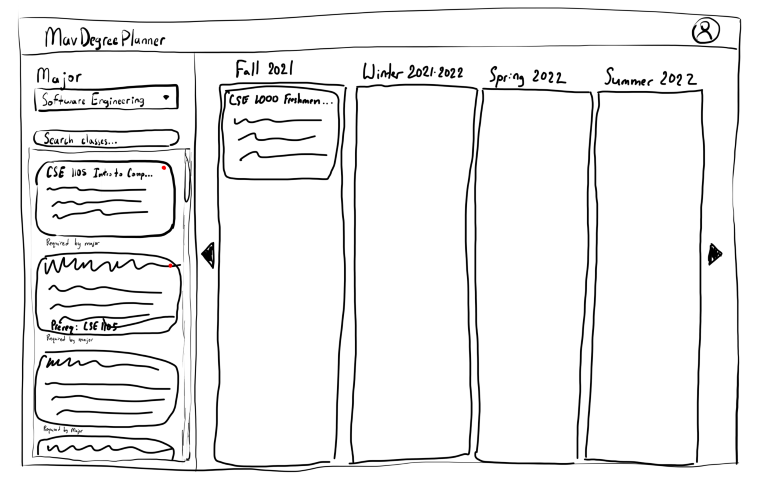
\includegraphics[width=0.5\textwidth]{images/MavDegreePlannerDiagram-Small} % Image
    \caption{Diagram of Major System Components} % Caption
\end{figure}